%%%%%%%%%%%%%%%%%%%%%%%%%%% asme2e.tex %%%%%%%%%%%%%%%%%%%%%%%%%%%%%%%
% Template for producing ASME-format articles using LaTeX            %
% Written by   Harry H. Cheng                                        %
%              Integration Engineering Laboratory                    %
%              Department of Mechanical and Aeronautical Engineering %
%              University of California                              %
%              Davis, CA 95616                                       %
%              Tel: (530) 752-5020 (office)                          %
%                   (530) 752-1028 (lab)                             %
%              Fax: (530) 752-4158                                   %
%              Email: hhcheng@ucdavis.edu                            %
%              WWW:   http://iel.ucdavis.edu/people/cheng.html       %
%              May 7, 1994                                           %
% Modified: February 16, 2001 by Harry H. Cheng                      %
% Modified: January  01, 2003 by Geoffrey R. Shiflett                %
% Use at your own risk, send complaints to /dev/null                 %
%%%%%%%%%%%%%%%%%%%%%%%%%%%%%%%%%%%%%%%%%%%%%%%%%%%%%%%%%%%%%%%%%%%%%%

%%% use twocolumn and 10pt options with the asme2e format
\documentclass[cleanfoot,cleanhead,onecolumn,12pt,notitlepage]{asme2e}
\special{papersize=8.5in,11in}

\usepackage{listings}
\usepackage{graphicx}
\usepackage{amsmath}
\usepackage[hidelinks]{hyperref}
\lstset{
    breaklines=true, % break lines for files
    basicstyle=\scriptsize,
    numbers=left,
    showstringspaces=false,
    frame=l
}

%% The class has several options
%  onecolumn/twocolumn - format for one or two columns per page
%  10pt/11pt/12pt - use 10, 11, or 12 point font
%  oneside/twoside - format for oneside/twosided printing
%  final/draft - format for final/draft copy
%  cleanfoot - take out copyright info in footer leave page number
%  cleanhead - take out the conference banner on the title page
%  titlepage/notitlepage - put in titlepage or leave out titlepage
%  
%% The default is oneside, onecolumn, 10pt, final

%%% You need to remove 'DRAFT: ' in the title for the final submitted version.
\title{Major Project \# 3}

%%% first author
\author{Shaun Harris
    \affiliation{
	Department of Mechanical and Aerospace Engineering\\
	Utah State University \\
    Email: shaun.r.harris@gmail.com
    }
}


\begin{document}

\maketitle    

%%%%%%%%%%%%%%%%%%%%%%%%%%%%%%%%%%%%%%%%%%%%%%%%%%%%%%%%%%%%%%%%%%%%%%

\begin{abstract}
    {\it A fixed Earth Gravity Cancellation (EGC) Rocket was examined.  The fuel type was considered both as a monopropellant and as a hybrid ABS rocket.  The fuel types were compared and examined and the resulting analysis and conclusions are presented here.}
\end{abstract}

\newpage

\tableofcontents

%%%%%%%%%%%%%%%%%%%%%%%%%%%%%%%%%%%%%%%%%%%%%%%%%%%%%%%%%%%%%%%%%%%%%%

\begin{nomenclature}
    \entry{$I_{sp}$}{Specific impulse of rocket (seconds)}
    \entry{$M_W$}{Molecular weight}
    \entry{$g_0$}{Gravity at sea level $9.806\ \frac{m}{s^2}$}
    \entry{$P_0$}{Stagnation Pressure (Pa)}
    \entry{$T_0$}{Stagnation Temperature or flame temperature (K)}
    \entry{$A_{exit}$}{Nozzle exit area}
    \entry{$A^*$ or $A_t$}{Nozzle throat area}
    \entry{$\frac{A_{exit}}{A_{t}}$}{exit area over throat area ratio}
    \entry{$t_2$}{time in seconds for ABS hybrid rocket fuel time}
    \entry{$t_1$}{time in seconds for Monopropellant rocket}
    \entry{$C^*$}{Characteristic velocity $(\frac{m}{s})$}
    \entry{$\dot{m}$}{Mass flow}
    \entry{$\frac{O}{F}$}{Oxidizer to Fuel ratio}
\end{nomenclature}

\newpage

\section{INTRODUCTION}

\subsection{Part 1}

The EGC rocket can use a hydrogen peroxide and water combination for the oxide and fuel.  This type of rocket is considered a monopropellant.  It can used at varying pressure values, and varying oxide to fuel ratios.  These ratios were examined and considered from 80\% to 99\%.  The nozzle outlet has a 4:1 nozzle exapansion.  NASA developed a code called CEA, this solver was used to calculate the various desired values for this case.  It calculated the Nozzle Exit Temperature, which was then compared to a separate calculated isentropic stagnation temperature.  The stagnation temperatures were calculated, and the nozzle exit and combuster temperatures were then compared.  The nozzle exit Mach number was calculated and shown from CEA.  The fuel to oxide ratio was then analyzed from the CEA output to show when all the water in the peroxide solution was completely vaporized with this nozzle and atmospheric pressure.  Based on a thrust level of 3114 $N$ the throat area was then calculated from the CEA output.  The corresponding $I_{sp}$ and $C*$ values were calculated.  The mass flow corresponding to this value was also calculated.

\subsection{Part 2}
The EGC rocket can also use an ABS mixture as the fuel, and the hydrogen peroxide and water as the oxidizers with varying ratios.  The optimal $C*$ values were considered as the optimal conditions.  The corresponding $I_{sp}$ and $\frac{O}{F}$ values were considered. The values of the hybrid rocket and the monopropellant were than compared.  

\subsection{Part 3}
The hover time of the EGC rocket were then considered.  The flight time was chosen to be the rocket consideration.  If the mass fraction is similar for each rocket, then Eq. \ref{eq:DVs} shows the relationship between flight time and $I_{sp}$ values.

\begin{equation}
    \begin{aligned}
        \Delta V_2 &= gt_2 = g_0 I_{sp2} ln(\frac{M_i}{M_f}) \\
        \Delta V_1 &= gt_1 = g_0 I_{sp1} ln(\frac{M_i}{M_f}) \\
        \frac{\Delta V_2 }{\Delta V_1} &= \frac{t_2}{t_1} = \frac{I_{sp2}}{I_{sp1}}
        \label{eq:DVs}
    \end{aligned}
\end{equation}


\section{RESULTS}


\subsection{Part 1}

The pressure was iterated upon until the resulting nozzle exit pressure was close to atmospheric pressure at sea level.  The chamber pressure was found to be approximately 28.5 bar.  With this pressure, CEA was simulated, and many of the calculations were used from the CEA output.  Section \ref{sec:A1} shows the configuration file used for the calculations.

The nozzle exit temperature and stagnation temperature were compared in the left part of Fig. \ref{fig:1-i}.  The plots x-axis shows the percent of mass concentration for the hydrogen peroxide.  We can see the nozzle exit temperature is significantly smaller than the stagnation temperature.  The right part of Fig. \ref{fig:1-i} shows the comparison of the combuster and nozzle exit stagnation temperatures.  These stagnation temperatures were calculated using isentropic relations.  


\begin{figure}[h!]
    \begin{center}
        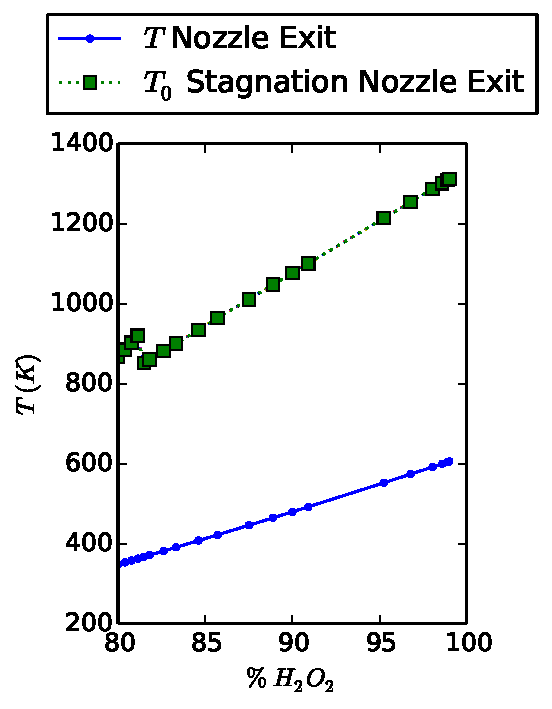
\includegraphics[width=0.45\linewidth]{../Plot_CEA/Part1/Part1_i.pdf}
        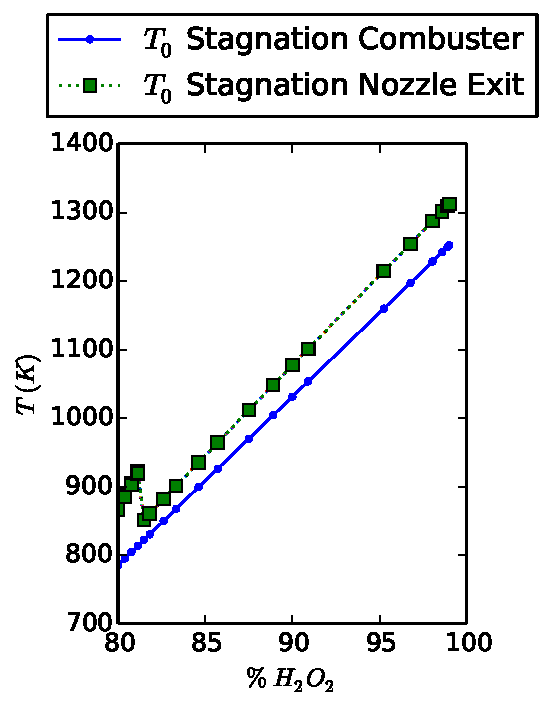
\includegraphics[width=0.45\linewidth]{../Plot_CEA/Part1/Part1_ii.pdf}
        \caption{Nozzle Exit and Combuster Stagnation Temperatures}
        \label{fig:1-i}
    \end{center}
\end{figure}

Fig. \ref{fig:1-iii} shows the nozzle exit Mach and characteristic velocity and thrust values.  Fig. \ref{fig:1-iv} shows the mass flow and $I_{sp}$ values.  It is noted that to get the correct specific impulse, we needed to convert from the European $I_{sp}$ values to the American standard in seconds by dividing by gravity at sea level.  The values at 9:1 ratio were used in the following comparisons.  


\begin{figure}[h!]
    \begin{center}
        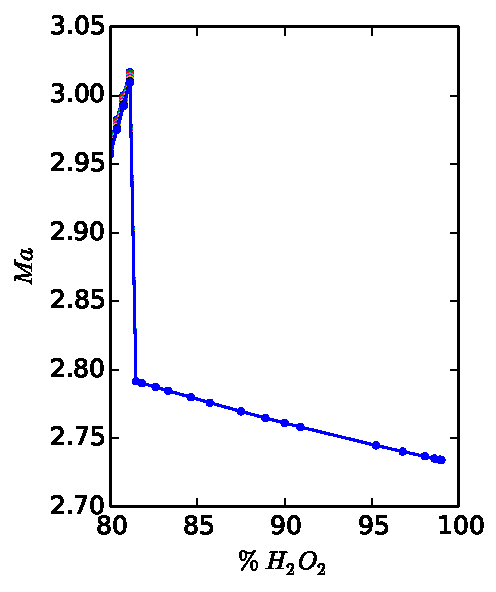
\includegraphics[width=0.45\linewidth]{../Plot_CEA/Part1/Part1_iii.pdf}
        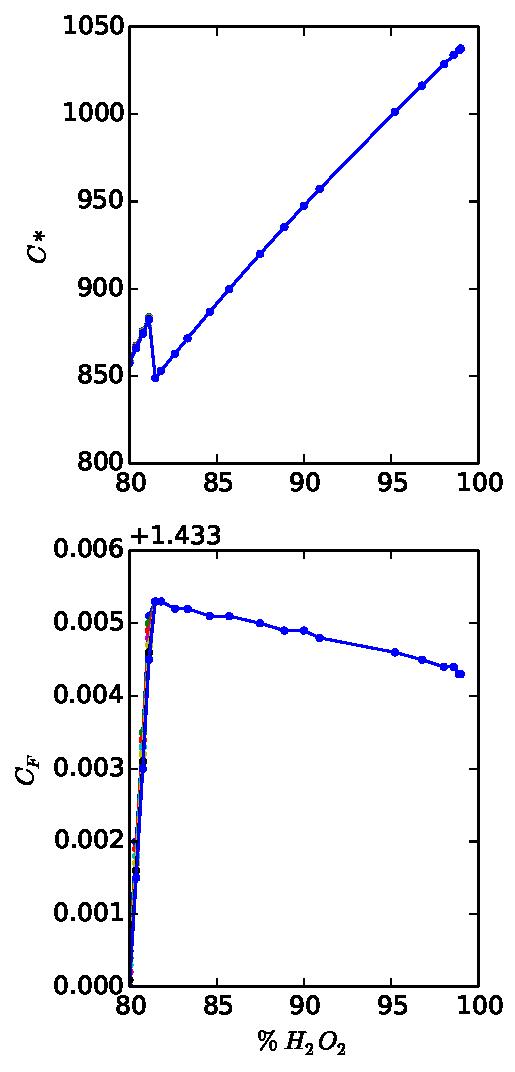
\includegraphics[width=0.45\linewidth]{../Plot_CEA/Part1/Part1_iv.pdf}
        \caption{Nozzle Exit Mach and $C^*$ and $C_F$ values}
        \label{fig:1-iii}
    \end{center}
\end{figure}


\begin{figure}[h!]
    \begin{center}
        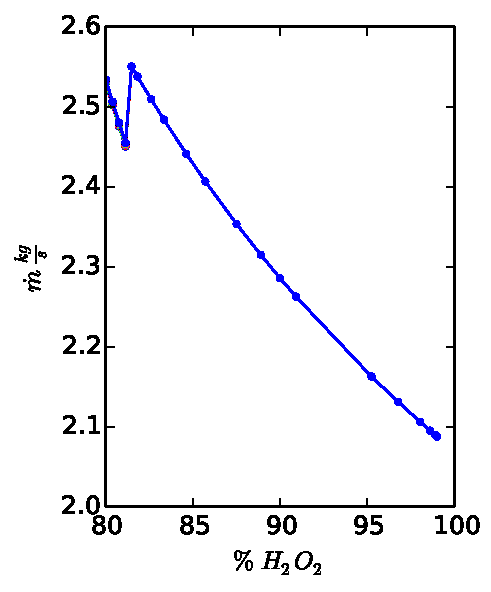
\includegraphics[width=0.45\linewidth]{../Plot_CEA/Part1/Part1_vi.pdf}
        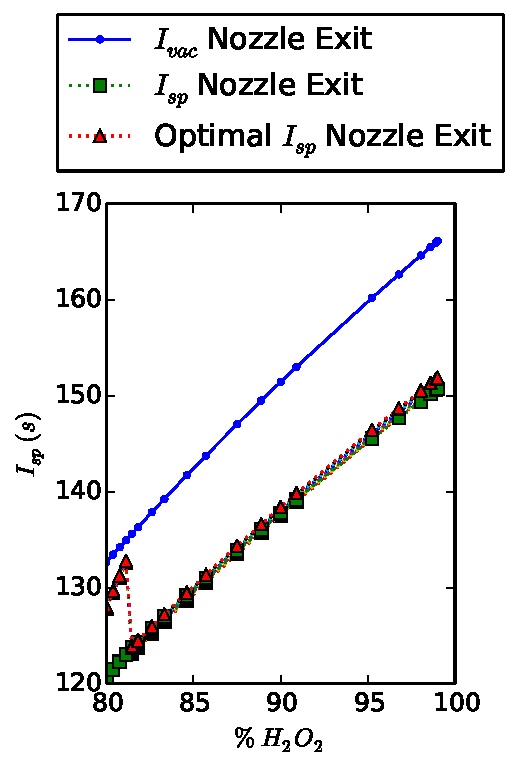
\includegraphics[width=0.45\linewidth]{../Plot_CEA/Part1/Part1_v.pdf}
        \caption{$I_{sp}$ values at the nozzle exit}
        \label{fig:1-iv}
    \end{center}
\end{figure}

Peroxide concentration requires a 5:1 Oxide to fuel ratio to vaporize all water
90\% $H_2O_2$ and optimal pressure gives:
\begin{itemize}
    \item \makebox[2cm]{at}         = 0.000807083035601
    \item \makebox[2cm]{isp}        = 137.823781358
    \item \makebox[2cm]{isp\_opt}   = 137.699990655
    \item \makebox[2cm]{mdot}       = 2.28586037785
\end{itemize}

\subsection{Part 2}

In order to calculate the various ABS simulations.  A configuration file similar to the one shown in Section \ref{sec:A2} was used.  The concentration of hydrogen peroxide and water was varied.  Five separate simulations were used where an 80\% hydrogen peroxide was increased by 5\% in each simulation.  The fifth simulation was run at 99\% concentration.  Each of the simulations varied in the $\frac{O}{F}$ ratio from 50\% to 99\%.  This yielded each simulation had an optimal condition.  This optimal condition was set as the largest $C^*$ value.  This optimal conditions appropriate output values were then shown in the following figures.

Fig. \ref{fig:2-c} shows the optimal $C^*$ value as a function of hydrogen peroxide concentration for each of the 5 simulations on the left.

\begin{figure}[h!]
    \begin{center}
        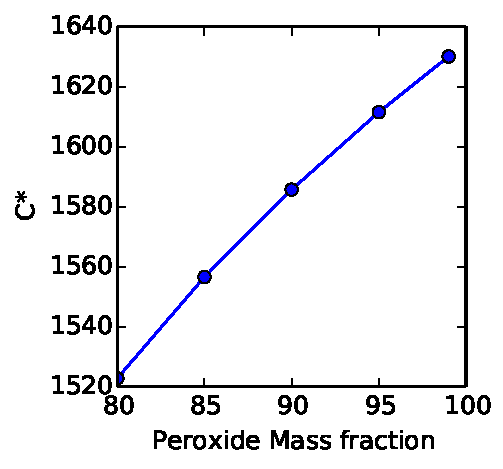
\includegraphics[width=0.45\linewidth]{../Plot_CEA/Part2/Part2_C_star.pdf}
        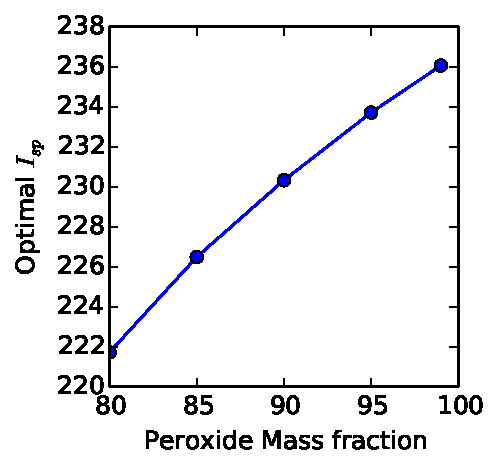
\includegraphics[width=0.45\linewidth]{../Plot_CEA/Part2/Part2_OptimalIsp.pdf}
        \caption{$C^*$ and $I_{sp}$ optimal values for each of the 5 simulations}
        \label{fig:2-c}
    \end{center}
\end{figure}

Fig. \ref{fig:2-c} also shows the optimal values from each of these simulations as a function of hydrogen peroxide concentration on the right.

Fig. \ref{fig:2-of} shows the optimal conditions $\frac{O}{F}$ ratio.  

\begin{figure}[h!]
    \begin{center}
        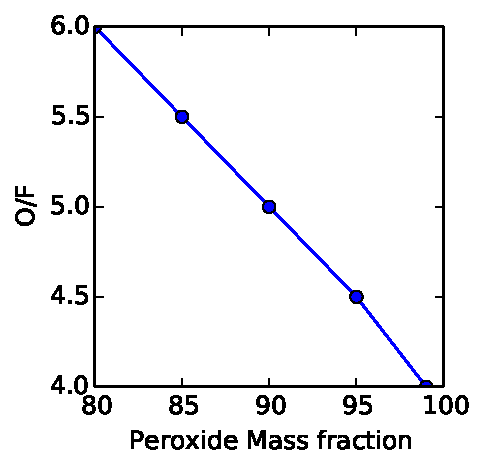
\includegraphics[width=0.45\linewidth]{../Plot_CEA/Part2/Part2_OF.pdf}
        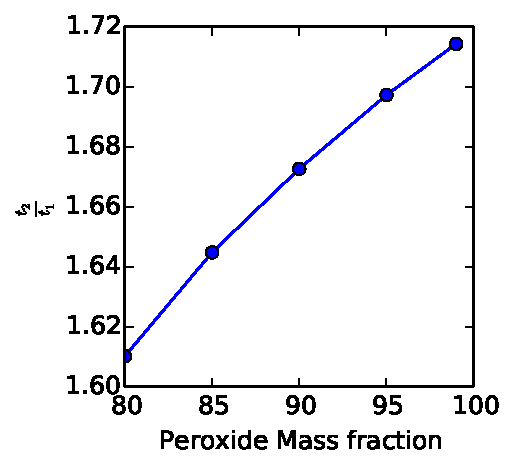
\includegraphics[width=0.45\linewidth]{../Plot_CEA/Part3/Part3.pdf}
        \caption{(left) The optimal O/F values are compared for each of the 5 simulations  (right) shows the time ratio of the hybrid rocket over the 90\% monopropellant}
        \label{fig:2-of}
    \end{center}
\end{figure}

\subsection{Part 3}

We desired to see the hover time of each of the rocket types considered and compare their respective abilities.  In order to do this, the ratio of $I_{sp}$ values were considered.  Eq. \ref{eq:DVs} was considered and the ratio was shown to relate to the ratio of hover time directly.  That is, assuming the vehicle mass fraction was the same.  We can see that at all simulation considered, the ABS hybrid rocket out performs the monopropellant rocket.  Fig. \ref{fig:3} shows the time ratio.  

It is important to note that the currently flight time of the EGC rocket is approximately 35 seconds.  Thus, the ratio could be used to calculate the flight time of the ABS hybrid rocket.  

\section{CONCLUSION}

We were able to show the advantage of using the ABS hybrid rocket in the EGC rocket motor.  With this in mind, we can see the cost effectiveness of using lower hydrogen peroxide solution to acheive better performance and longer hovering time.  If this motor is able to acheive the assumed mass fraction, then this could lead to a market disrupter in rocket engineering.  


%%%%%%%%%%%%%%%%%%%%%%%%%%%%%%%%%%%%%%%%%%%%%%%%%%%%%%%%%%%%%%%%%%%%%%

%\bibliographystyle{asmems4}
%\bibliography{asme2e}

%%%%%%%%%%%%%%%%%%%%%%%%%%%%%%%%%%%%%%%%%%%%%%%%%%%%%%%%%%%%%%%%%%%%%%

%
%%%%%%%%%%%%%%%%%%%%%%%%%%%%%%%%%%%%%%%%%%%%%%%%%%%%%%%%%%%%%%%%%%%%%%

\appendix

\section{Appendix A: Plotting Code}
\label{sec:code}

\subsection{Part 1 configuration file}
\label{sec:A1}
\lstinputlisting{../CEAexec/Part1_try1.inp}

\subsection{Part 2 configuration file}
\label{sec:A2}
\lstinputlisting{../CEAexec/Part2_try1.inp}

\subsection{Plotting python script}
\lstinputlisting[language=python]{../Plot_CEA/plot_stuff.py}





\end{document}
